\documentclass[presentation]{beamer}
\usepackage[utf8]{inputenc}
\usepackage{graphicx}
\usepackage{amsmath}
\usepackage{amssymb}
\usepackage{mathtools}
\mathtoolsset{showonlyrefs}
% \usetheme{simple}
\usepackage{array}
\usepackage{textcomp}
\newcommand{\textapprox}{\raisebox{0.5ex}{\texttildelow}}

\author{Scott Trinkle}
\date{November 15, 2017}
\title{Update on Dual Energy Phase Contrast}

\begin{document}

\frame{\titlepage}

\begin{frame}{Model}

  Measured intensity:
  
  \begin{align}
    I_R^{(j)} &= \int w(E) I_0^{(j)}(E) T(E) \left(1 + \frac{R_2}{k(E)} \nabla^2 \phi(E)\right)dE
  \end{align}

  with:\newline

  \begin{tabular}{c l}
    $w(E)$ & detector response [$\approx E$]\\
    $I_0^{(j)}$ & entrance intensity for spectrum $j$ [photons/s/0.1\%BW/mrad$^2$]\\
    $T(E)$ & transmission factor [unitless]\\
    $R_2$ & sample-detector distance [$\approx$30 cm]\\
    $k(E)$ & wave number [$\frac{2\pi}{\lambda(E)} \approx 10^{11}$ m]\\
    $\phi(E)$ & phase factor [unitless]
  \end{tabular}


\end{frame}

\begin{frame}{Spectra: $I_0^{(j)}(E) \approx 10^{13}$}

  \centering
  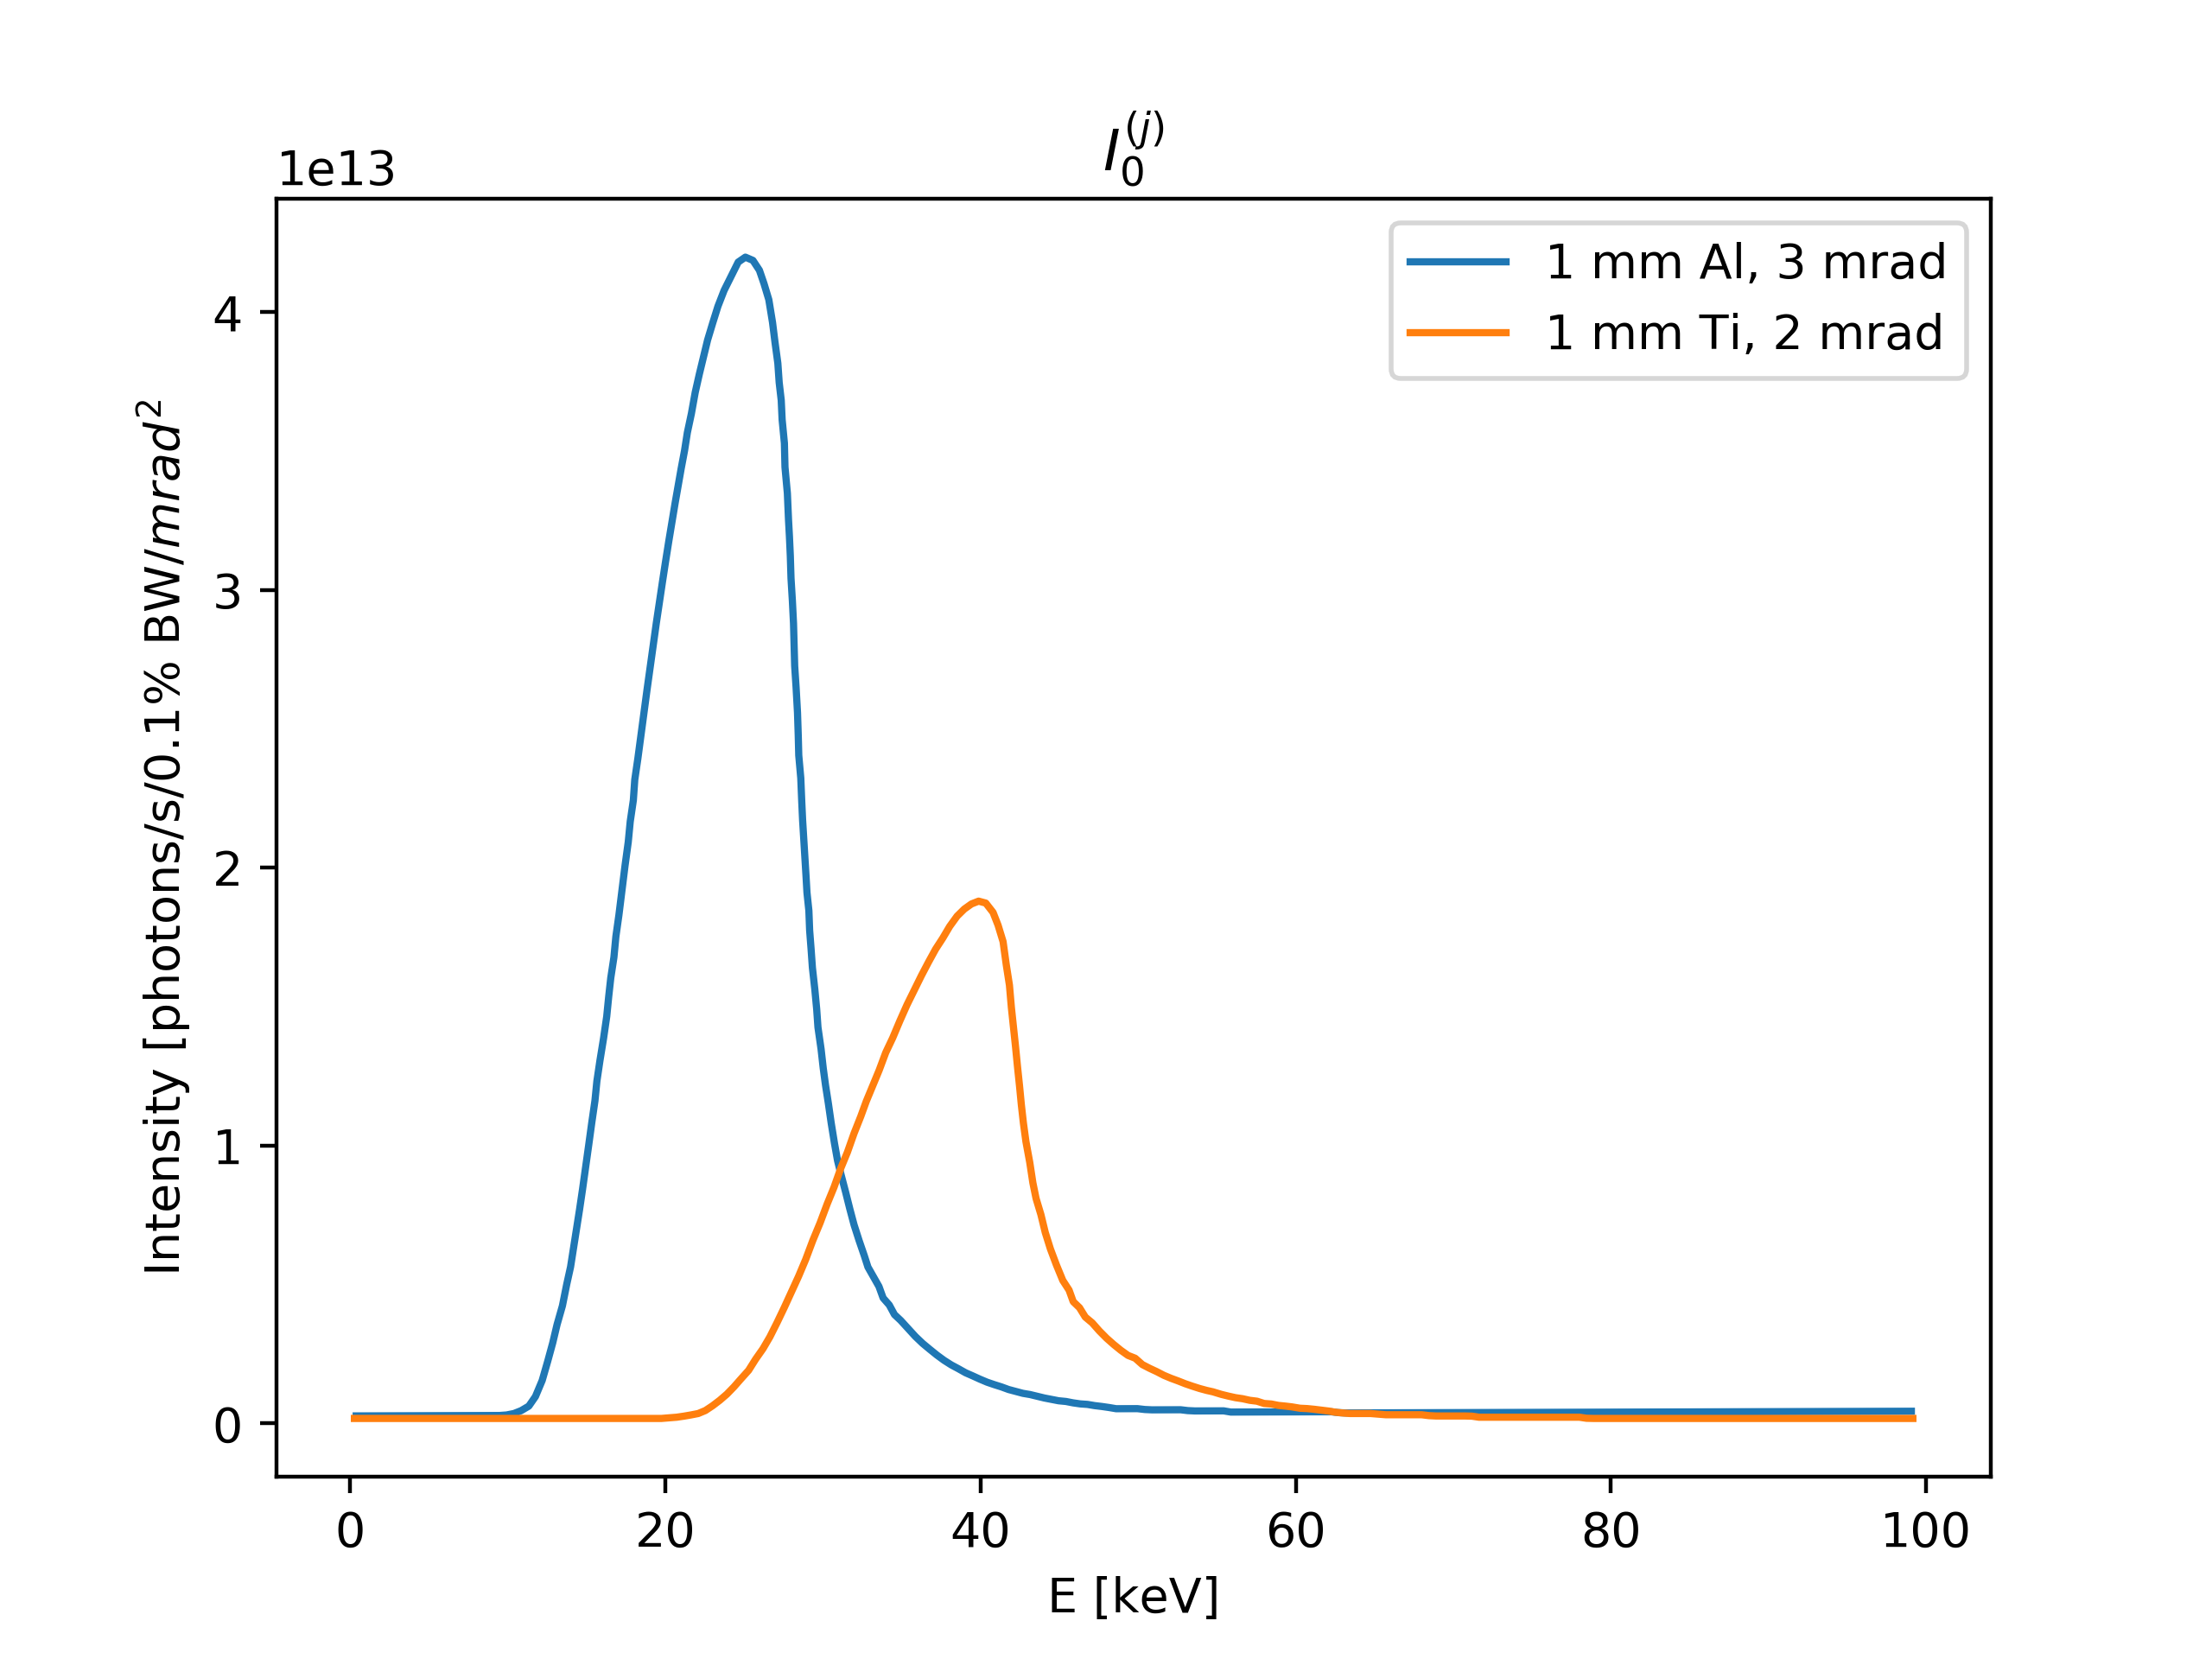
\includegraphics[width=0.8\linewidth]{figs/spectra}

\end{frame}

\begin{frame}{$\phi(E)$ and $T(E)$}
  \begin{align}
    \phi(E) &= r_e \lambda(E) \sum_i f_1^{(i)}(E) \int_L n_{a,i}(\vec{x})dl\\[6pt]
    T(E) &= \text{exp}\left(-2r_e \lambda(E) \sum_i f_2^{(i)}(E) \int_L n_{a,i}(\vec{x})dl\right)\\
  \end{align}

  with:\newline

  \begin{tabular}{c l}
    $r_e$ & classical electron radius [$\approx 10^{-15}$ m]\\
    $\lambda(E)$ & wavelength [$\approx 10^{-11} - 10^{-9}$ m]\\
    $f_1$, $f_2$ & oscillation modes per atom [$\approx 10^{1}-10^{2}$ atom$^{-1}$]\\
    $n_{a,i}(\vec{x})$ & ``atomic'' number density [atoms / cm$^3$]
  \end{tabular}
  
\end{frame}

\begin{frame}{$f_1$ and $f_2$ from NIST}

  \centering
  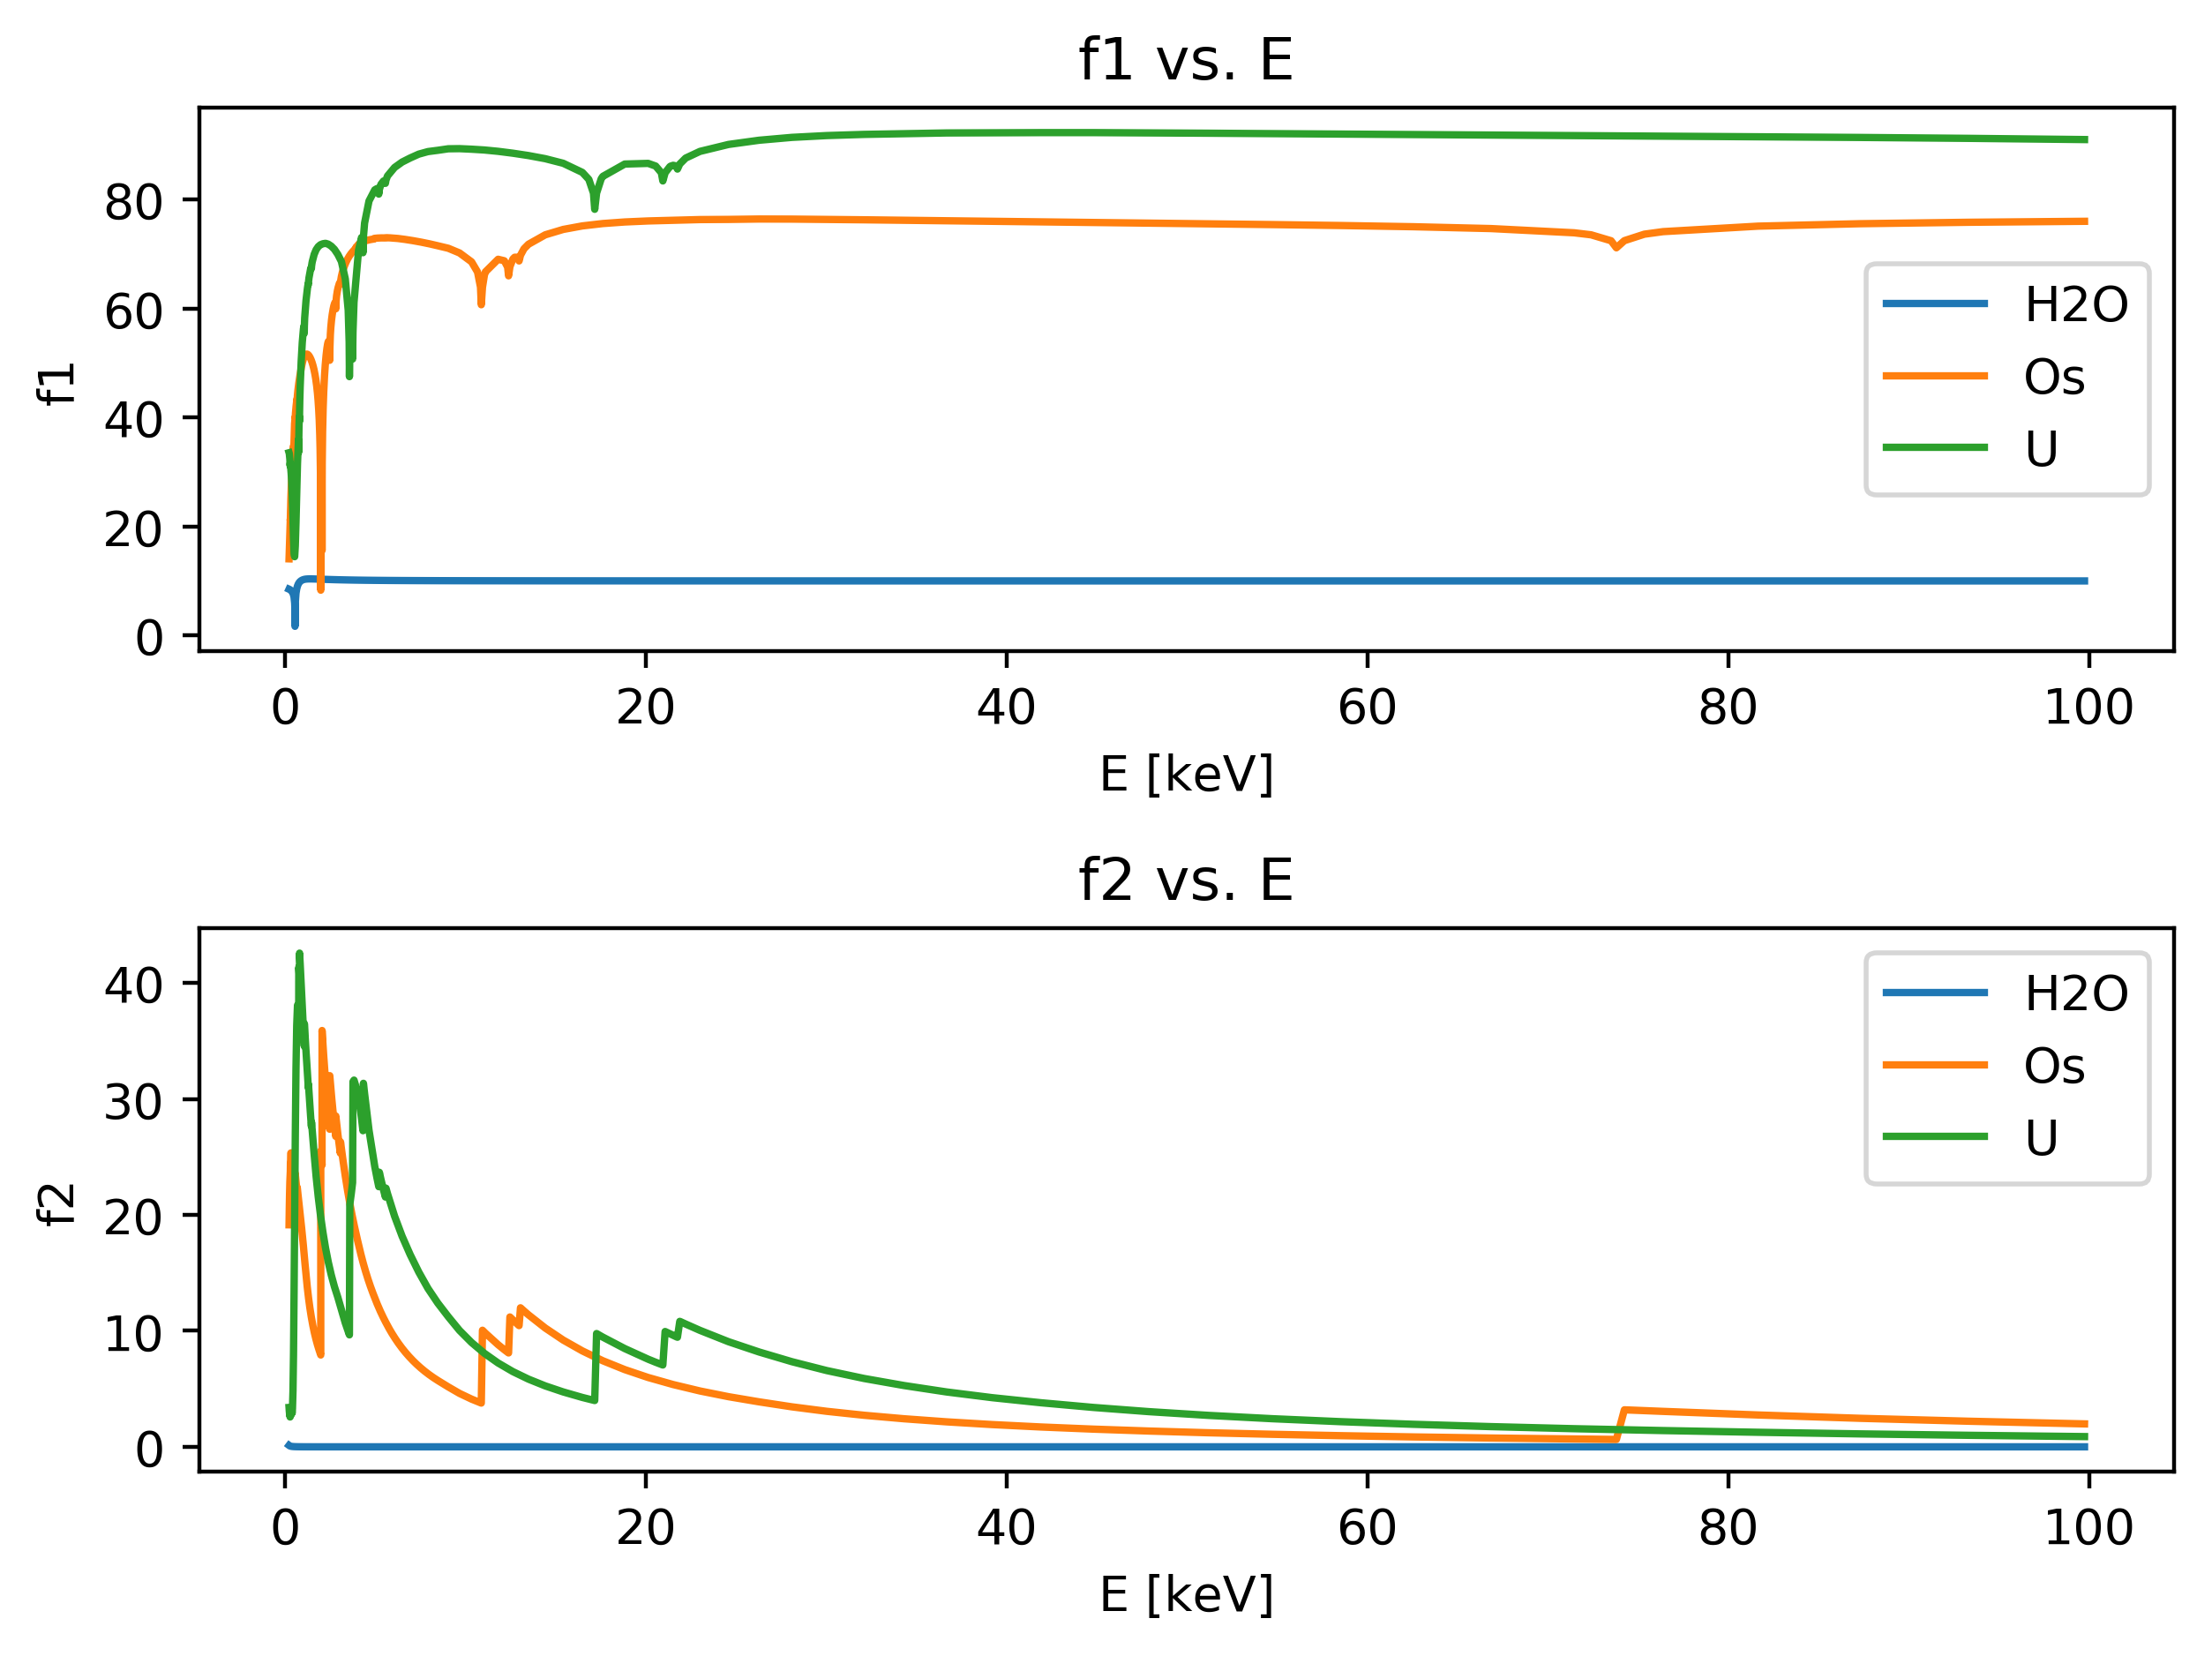
\includegraphics[width=0.8\linewidth]{figs/f1_f2}

\end{frame}

\begin{frame}{H$_2$O and Metal Phantoms}
  \begin{center}
    \begin{tabular}{m{5em} m{8cm}}
      Al filter & 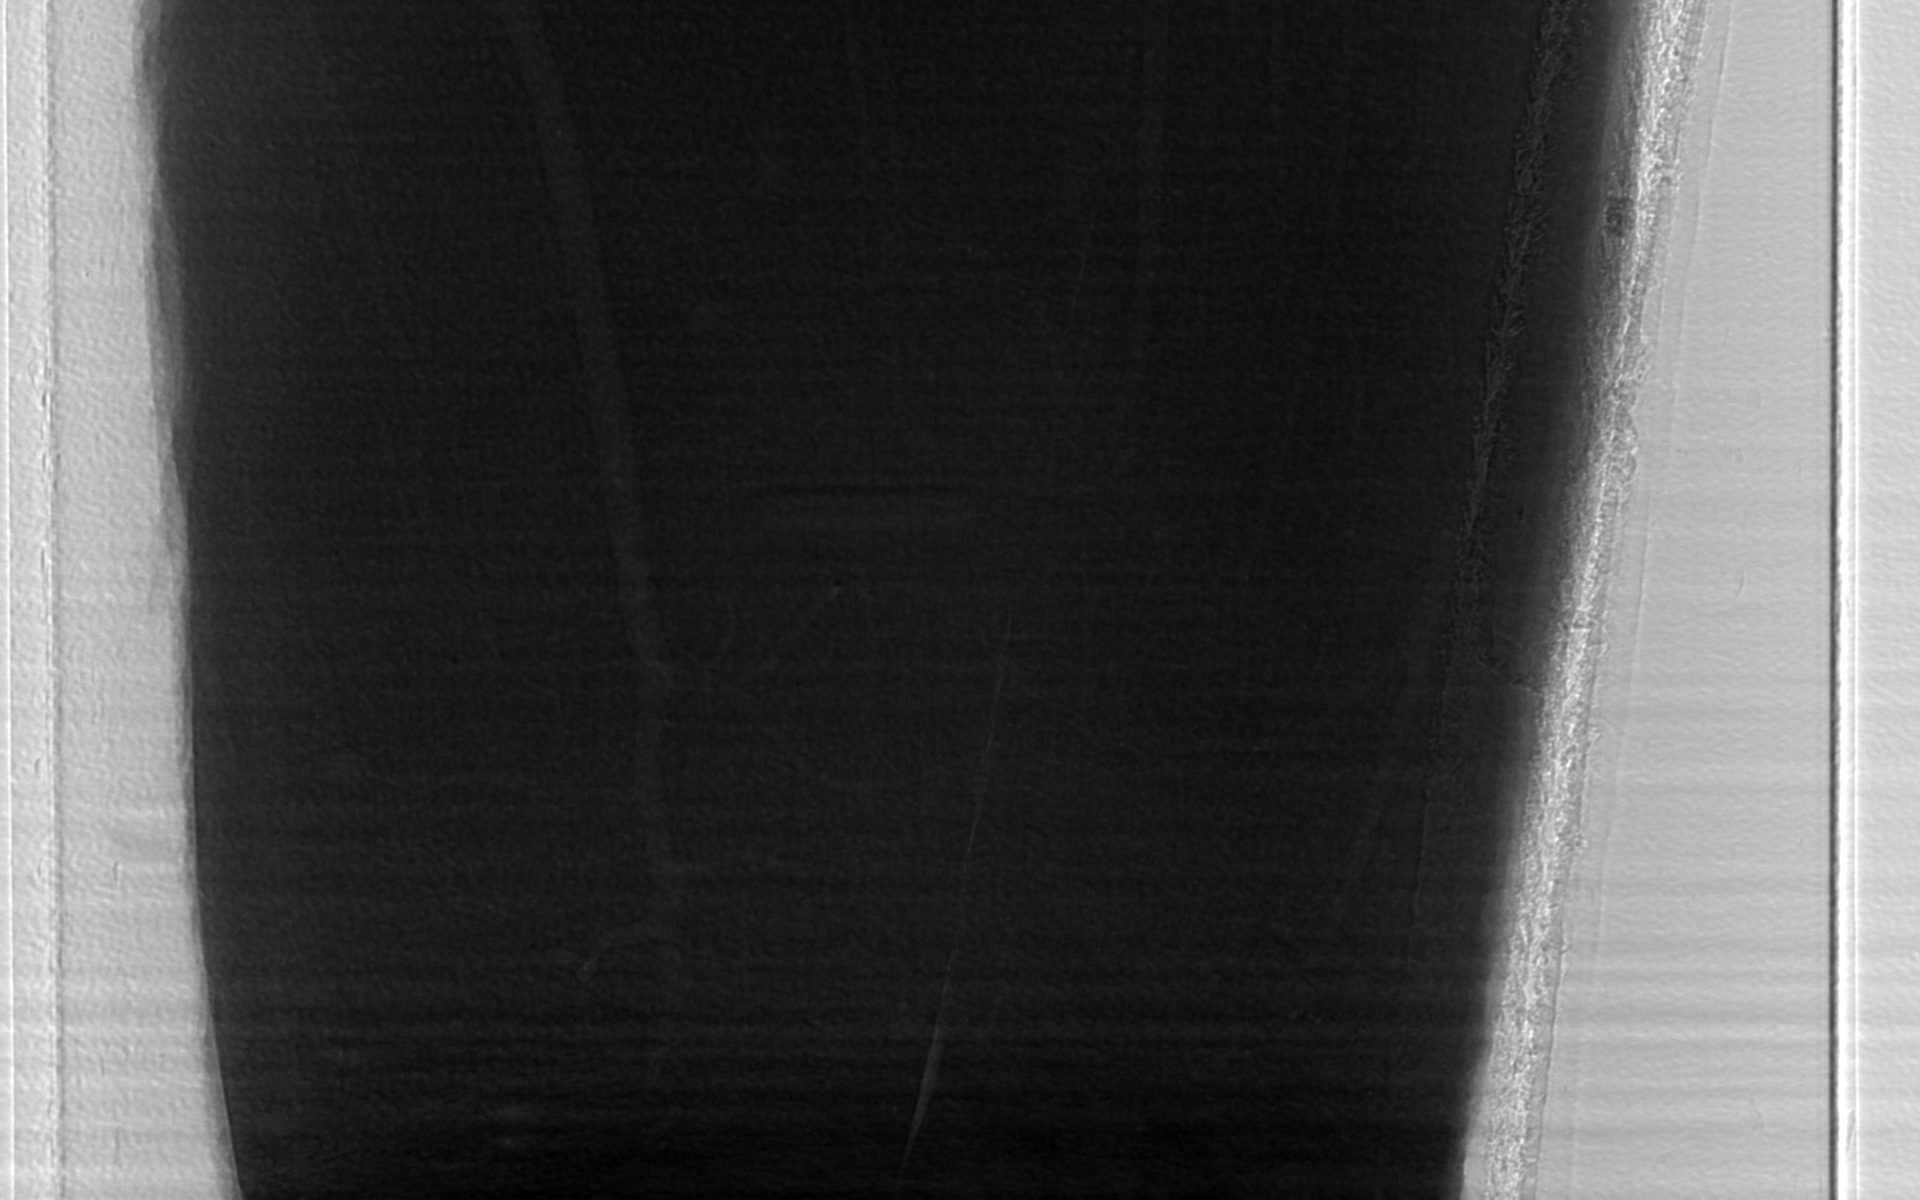
\includegraphics[width=6cm]{figs/Al_1080}\\
      No filter & 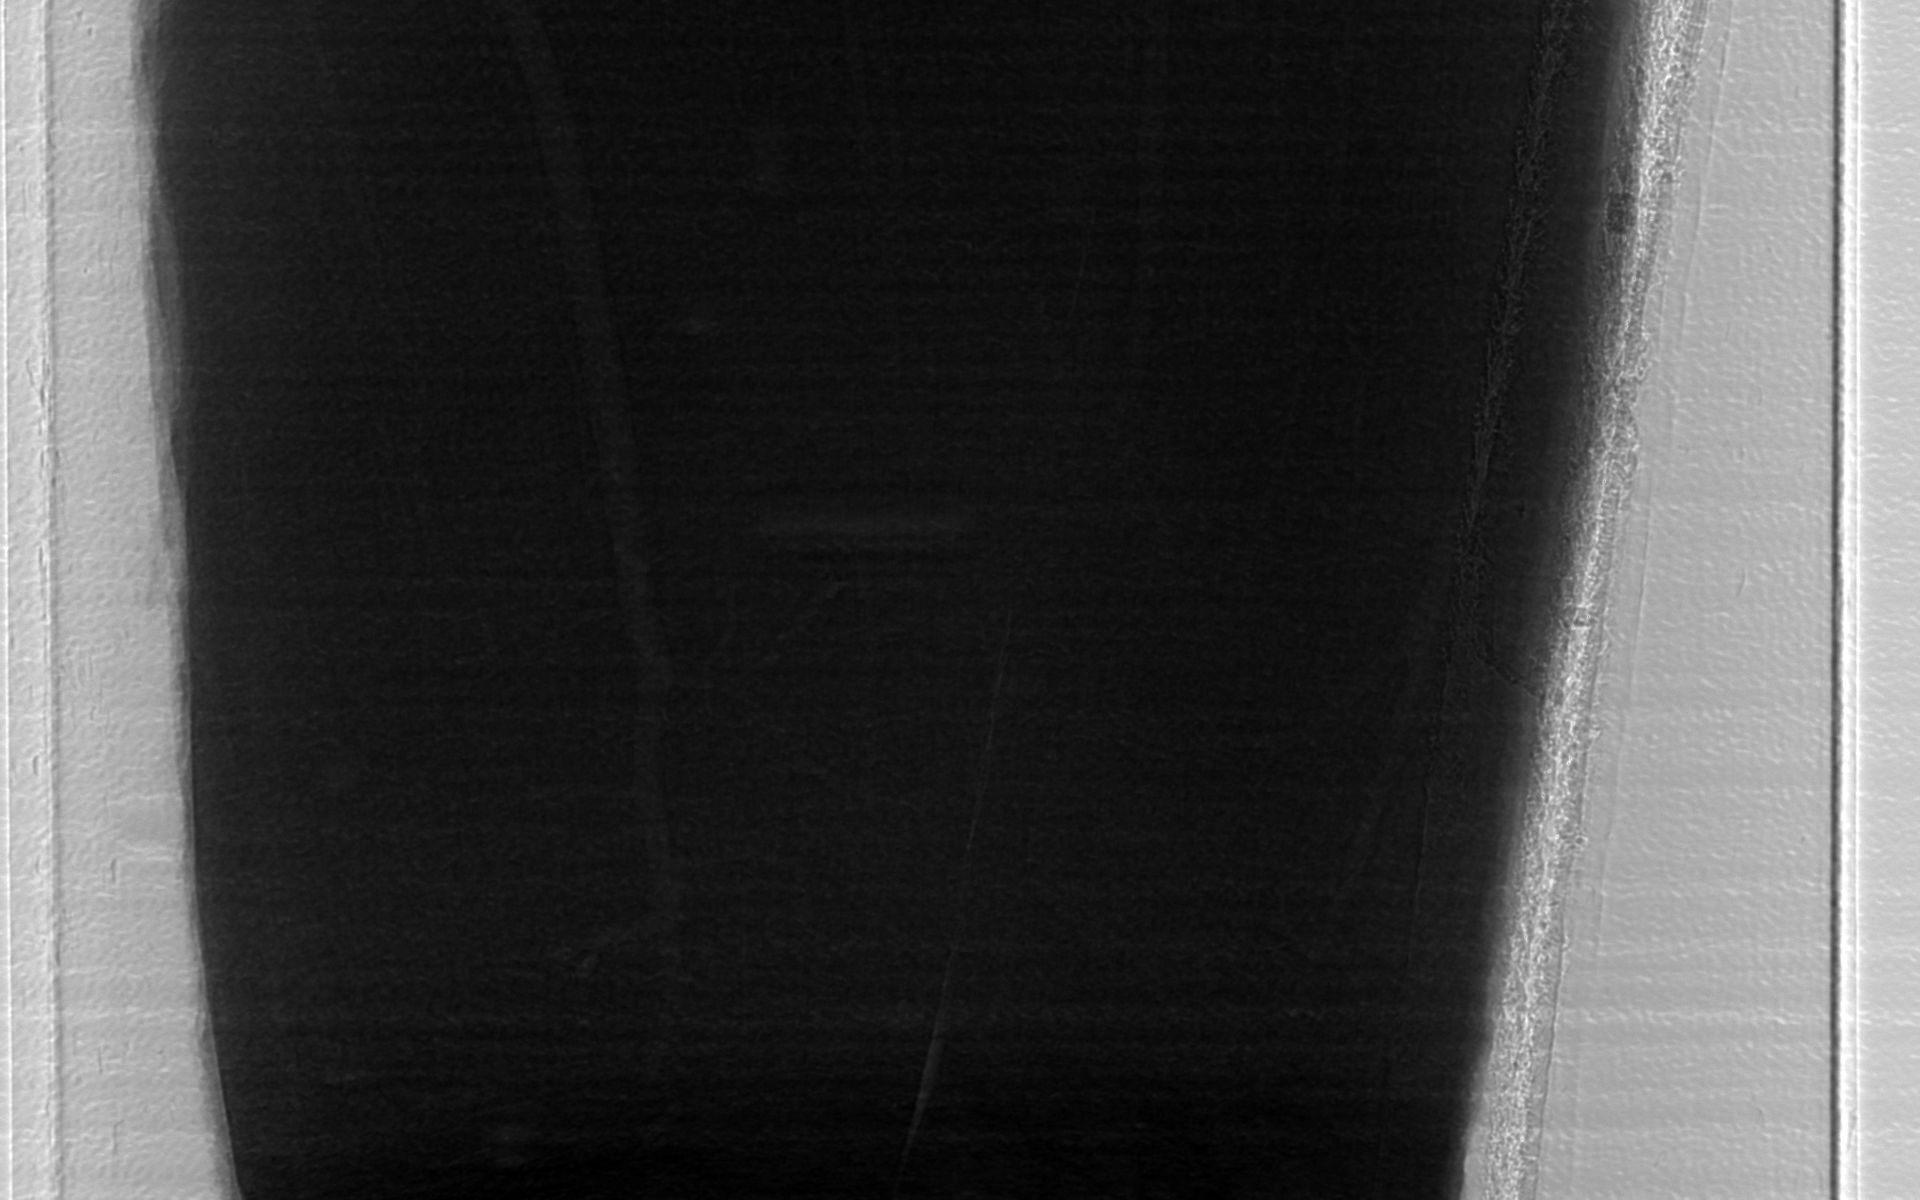
\includegraphics[width=6cm]{figs/No_1080}
    \end{tabular}
  \end{center}
\end{frame}


\begin{frame}{$\int_L n_{a,i}(\vec{x}) dl$}

  Normalized phantom images by number densities:
  \begin{align}
    \int_L n_{a,i}(\vec{x}) dl &\approx \frac{\rho_i N_a}{A_i} \Delta L * \left(\frac{\text{ph}_i(\vec{x})}{\text{mean}\{\text{ph}_i(\vec{x})\}}\right)\\
                               &\approx 10^{25} \text{ [cm}^{-2}]
  \end{align}

  \begin{table}
    \centering
    \begin{tabular}{l |c c c}
      & H$_2$O & U & Os\\\hline
      $\rho$ [g/cm$^{3}$] & 1.0 & 19.1 & 22.59\\
      A [g/mol] & 18.03 & 238.03 & 190.23\\
    \end{tabular}      
  \end{table}

  \centering
  $N_a = 6.022e23$ atoms/mole

  $\Delta L = 2.38$ mm

  

\end{frame}

\begin{frame}{$\nabla^2\int_L n_{a,i}(\vec{x}) dl$}

  \centering
  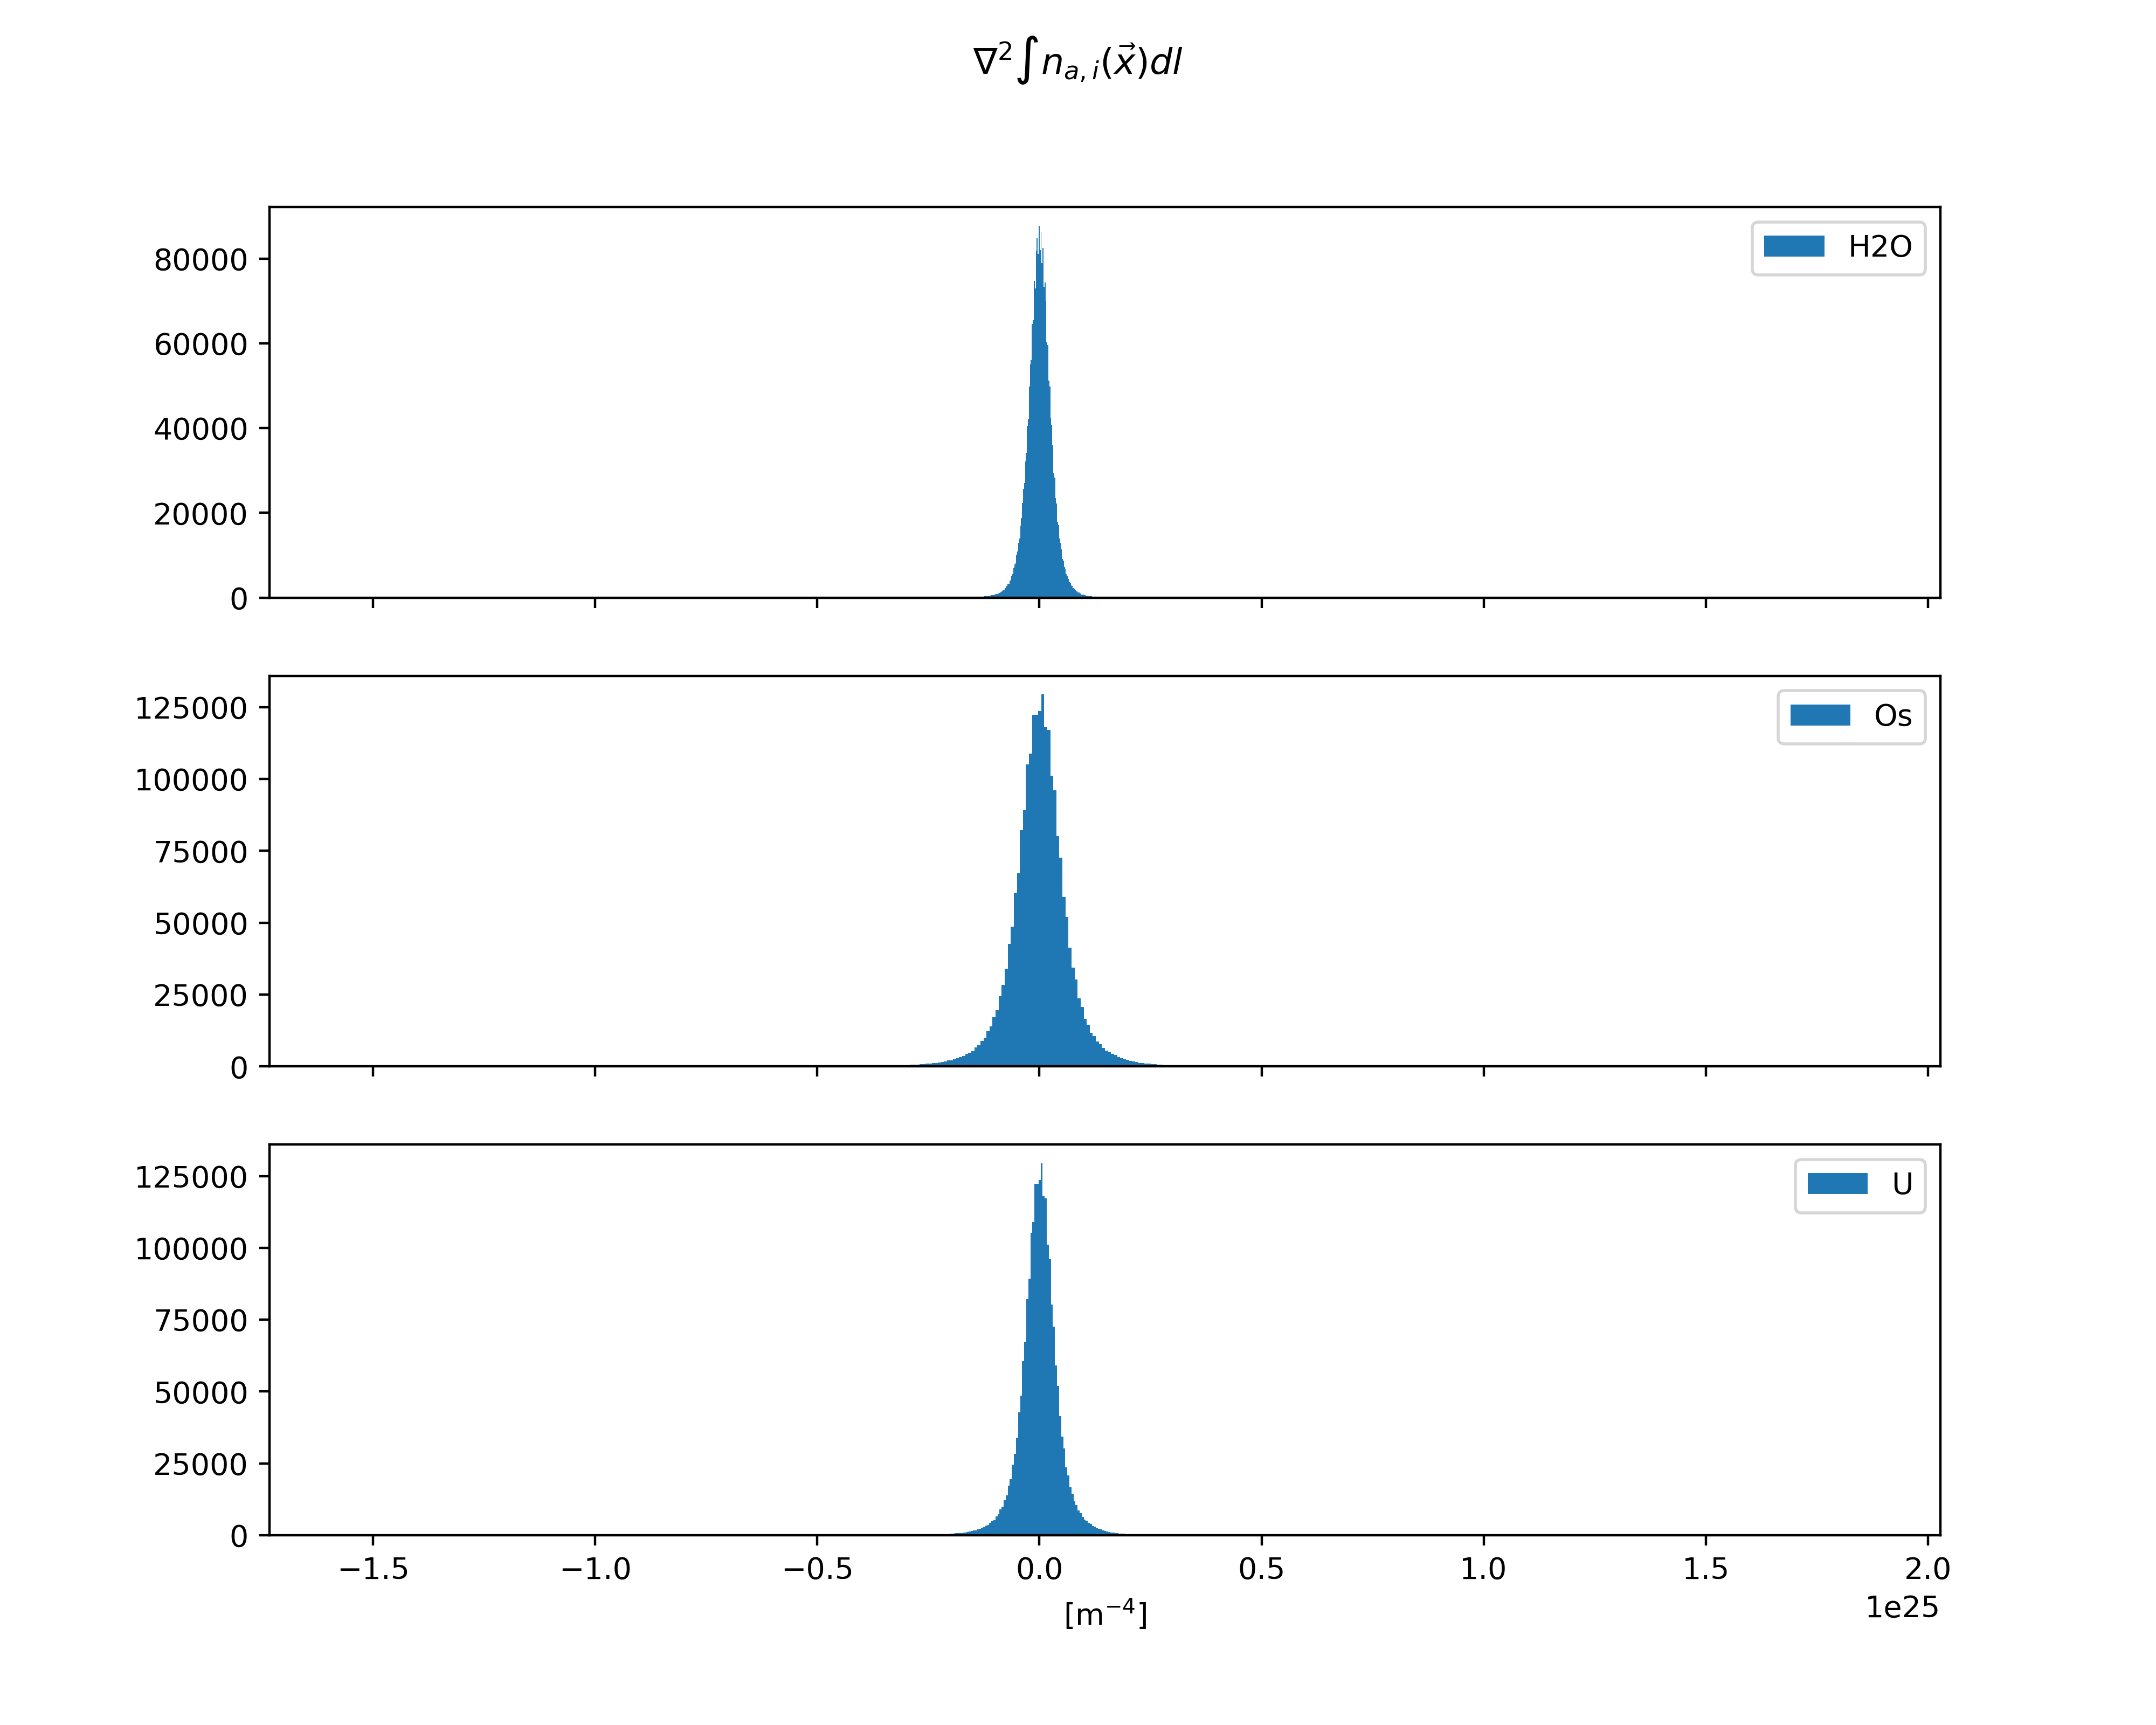
\includegraphics[width=0.75\linewidth]{figs/laplacians}

  \begin{tabular}{l | c c c}
    & H$_2$O & Os & U\\
    \hline
    Mean & 4e5 & 1e6 & -1e6\\
    Absolute value mean: & 2e23 & 5e23 & 3e23\\
    Max: & 4e24 & 2e25 & 1e25
  \end{tabular}  
    
\end{frame}

\begin{frame}
  \begin{align}
    \nabla^2 \phi(E) &= r_e \lambda(E) \sum_i f_1^{(i)}(E) \left[\nabla^2 \int_L n_{a,i}(\vec{x})dl\right]\\
                     &\approx [10^{-15} \text{ m}][10^{-11} - 10^{-9} \text{ m}][10^2][10^{6} - 10^{25} \text{ m}^{-4}]\\
                     &\approx 10^{-18} - 10^{3} \text{ m}^{-2}
  \end{align}

  \end{frame}

  \begin{frame}{$\nabla^2 \phi(E)$}

    \centering
    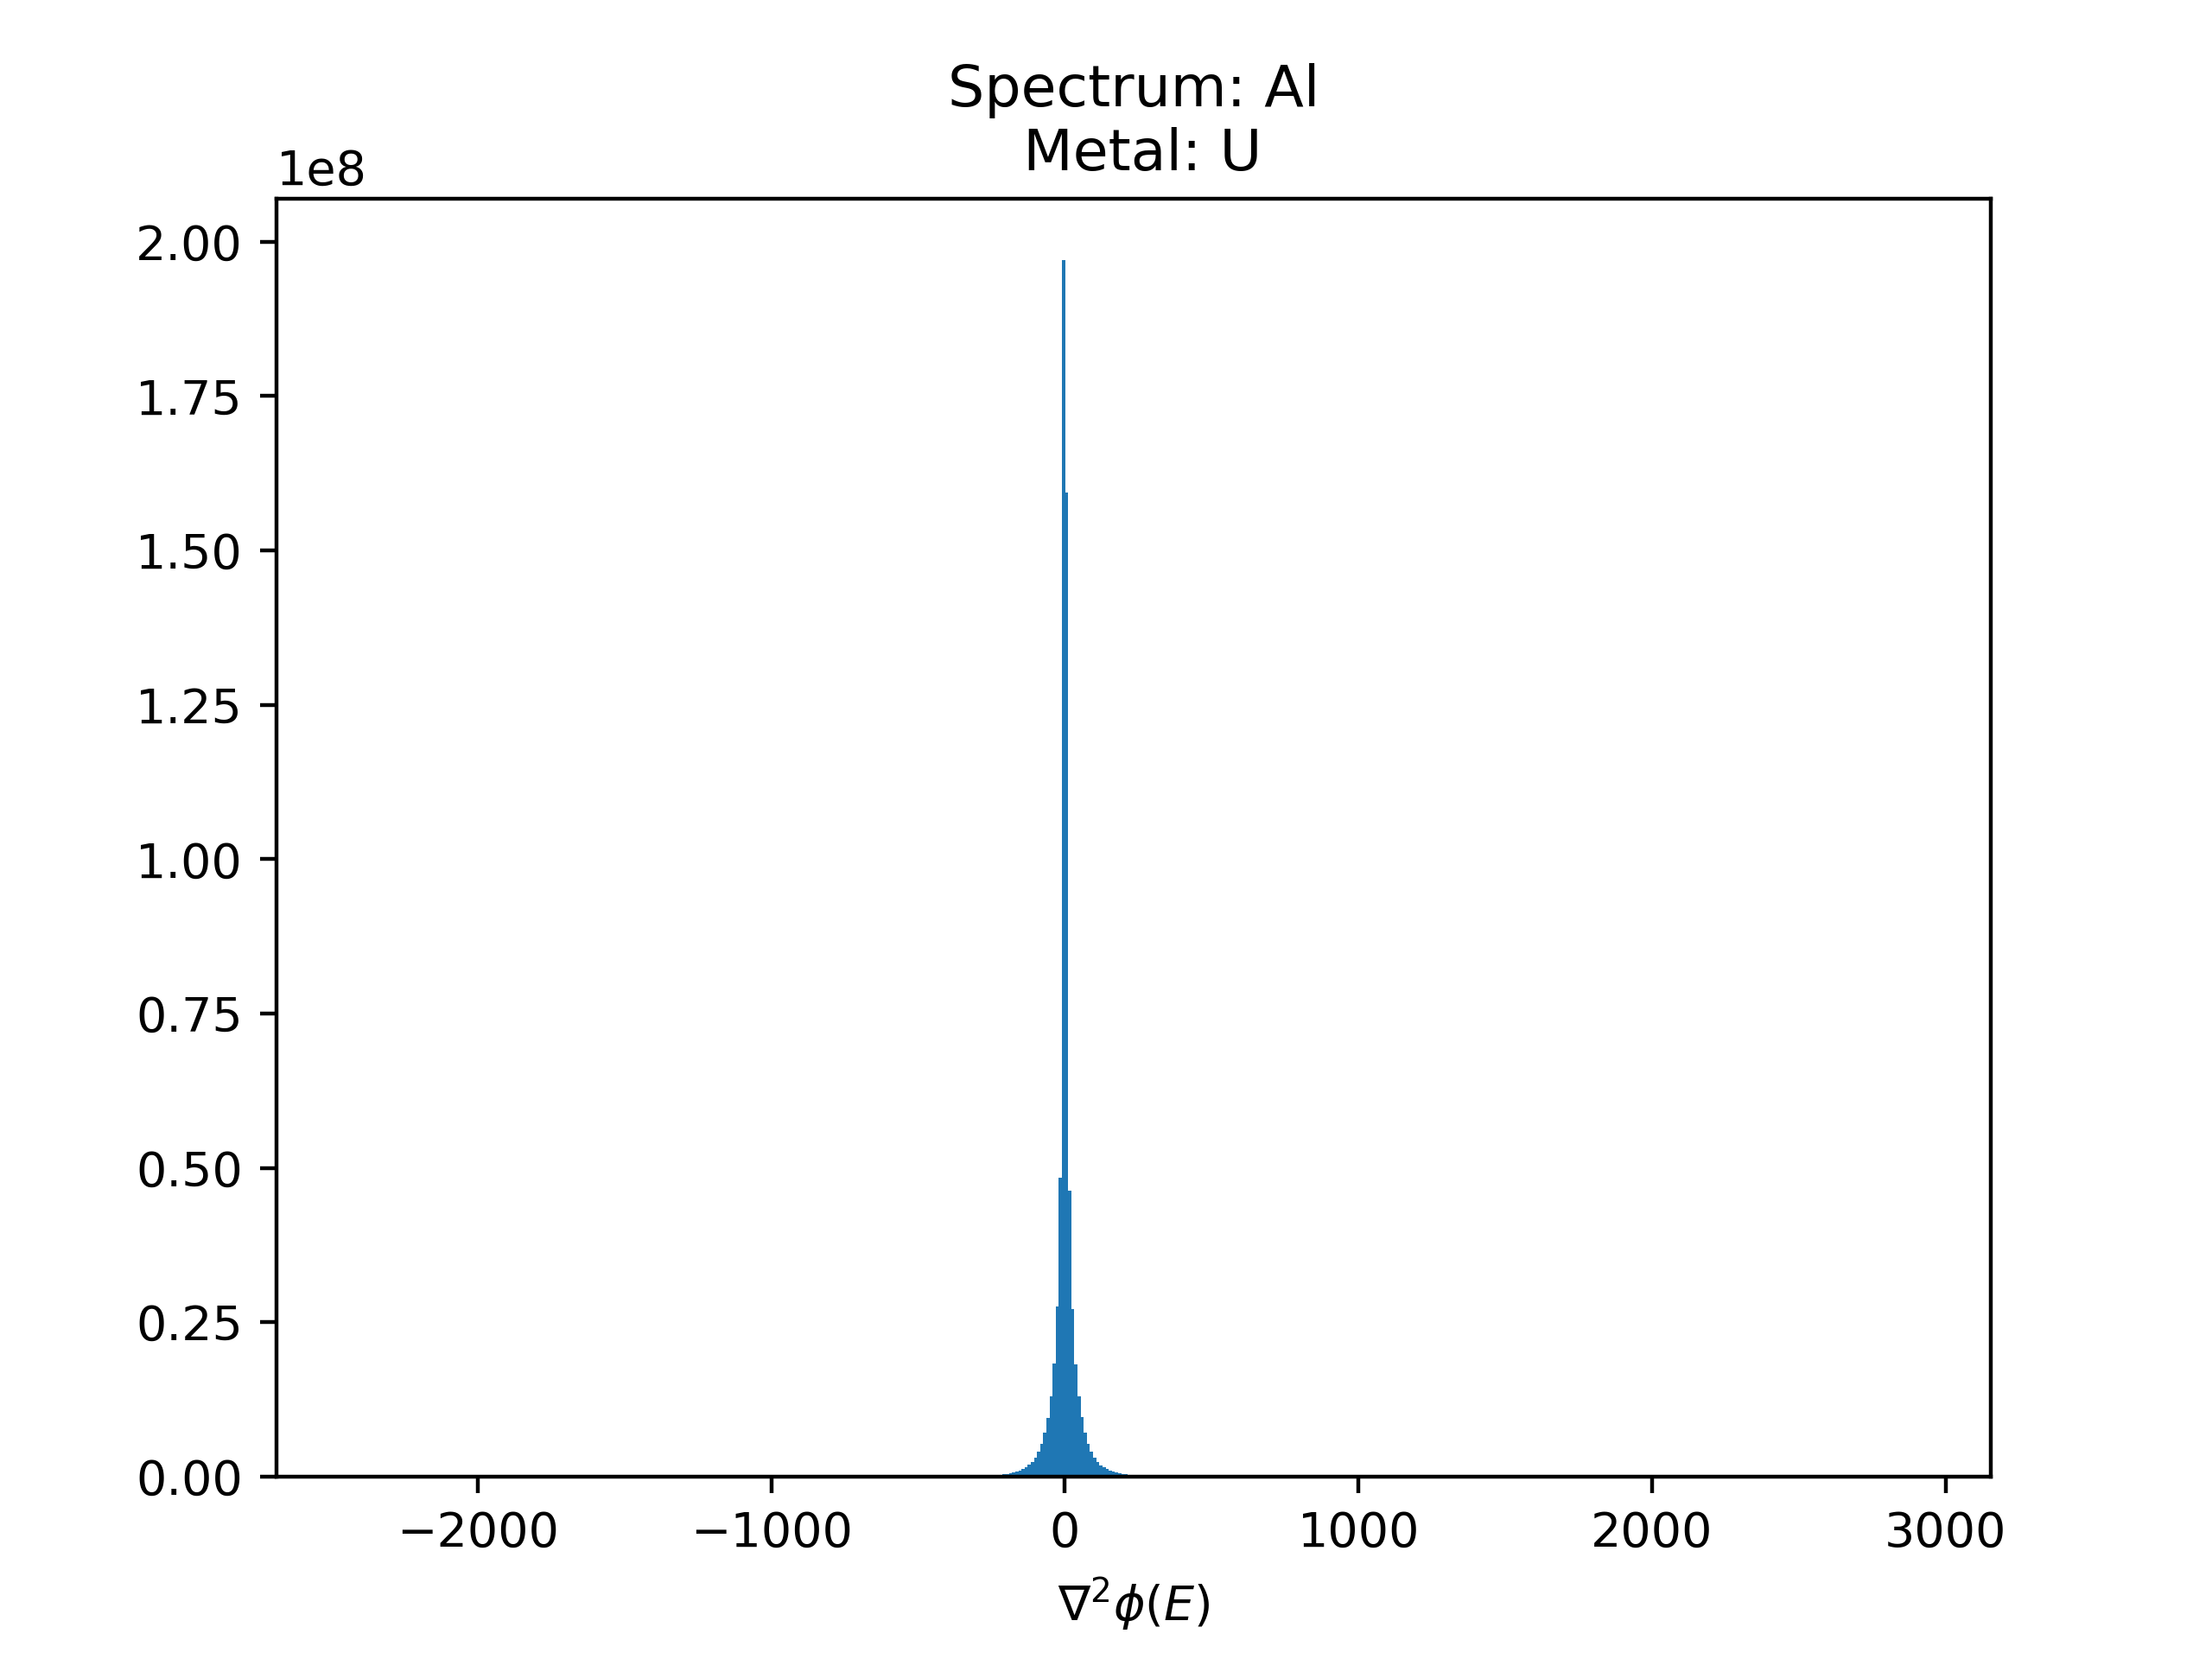
\includegraphics[width=0.8\linewidth]{figs/lap_phi}
  \end{frame}

  \begin{frame}{Issue: Small phase term}
    Recall: 

    \begin{equation}
      I_R^{(j)} = \int w(E) I_0^{(j)}(E) T(E) \left(1 + \frac{R_2}{k(E)} \nabla^2 \phi(E)\right)dE
    \end{equation}

    Phase term:
    
    \begin{align}
      &\frac{R_2}{k(E)}\nabla^2 \phi(E)\\
      &\approx \frac{[10^1 \text{ m}]}{[10^{11} \text{ m}^{-1}]}\cdot [10^{3} \text{ m}^{-2}]\\
      &\approx 10^{-7}
    \end{align}
    
  \end{frame}

  \begin{frame}{Issue: Small phase term}
    \centering
    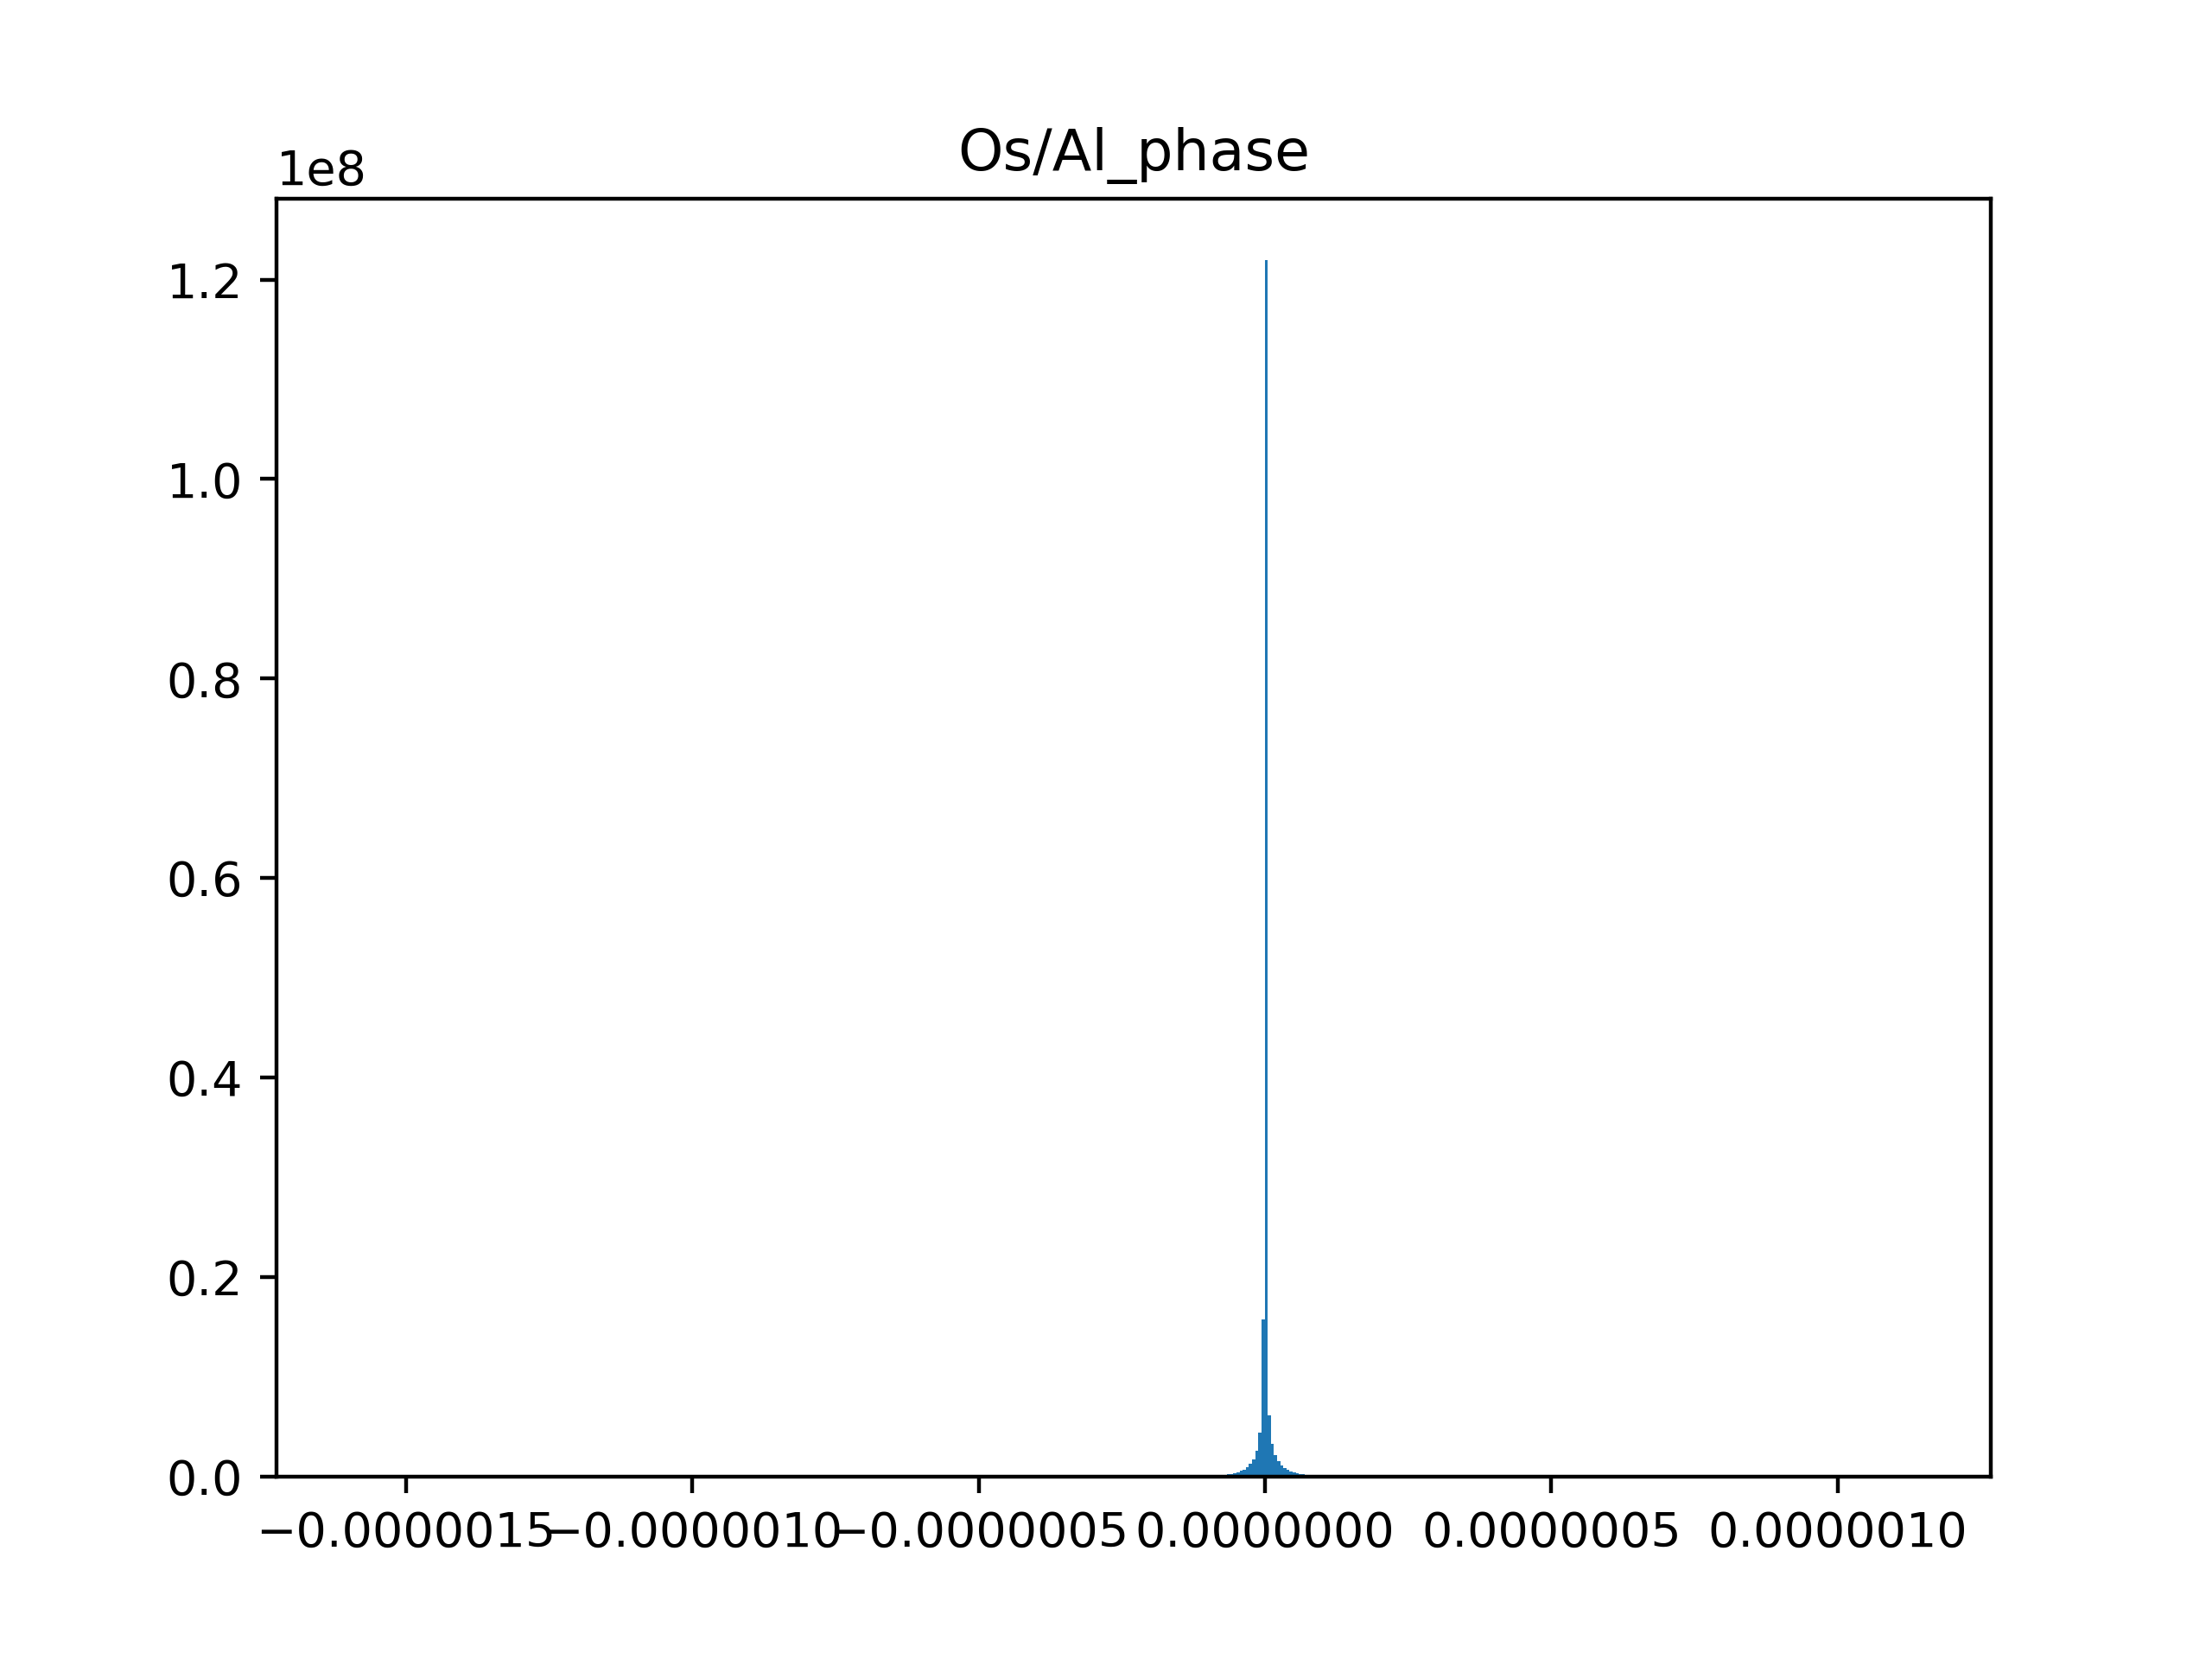
\includegraphics[width=0.8\linewidth]{figs/Al_phase}

  \begin{tabular}{l | c }
    Mean & 7e-26\\
    Absolute value mean: & 6e-9\\
    Max: & 1e-6\\
  \end{tabular}  

    
  \end{frame}

  \begin{frame}{Issue: Small phase term}
    \centering
    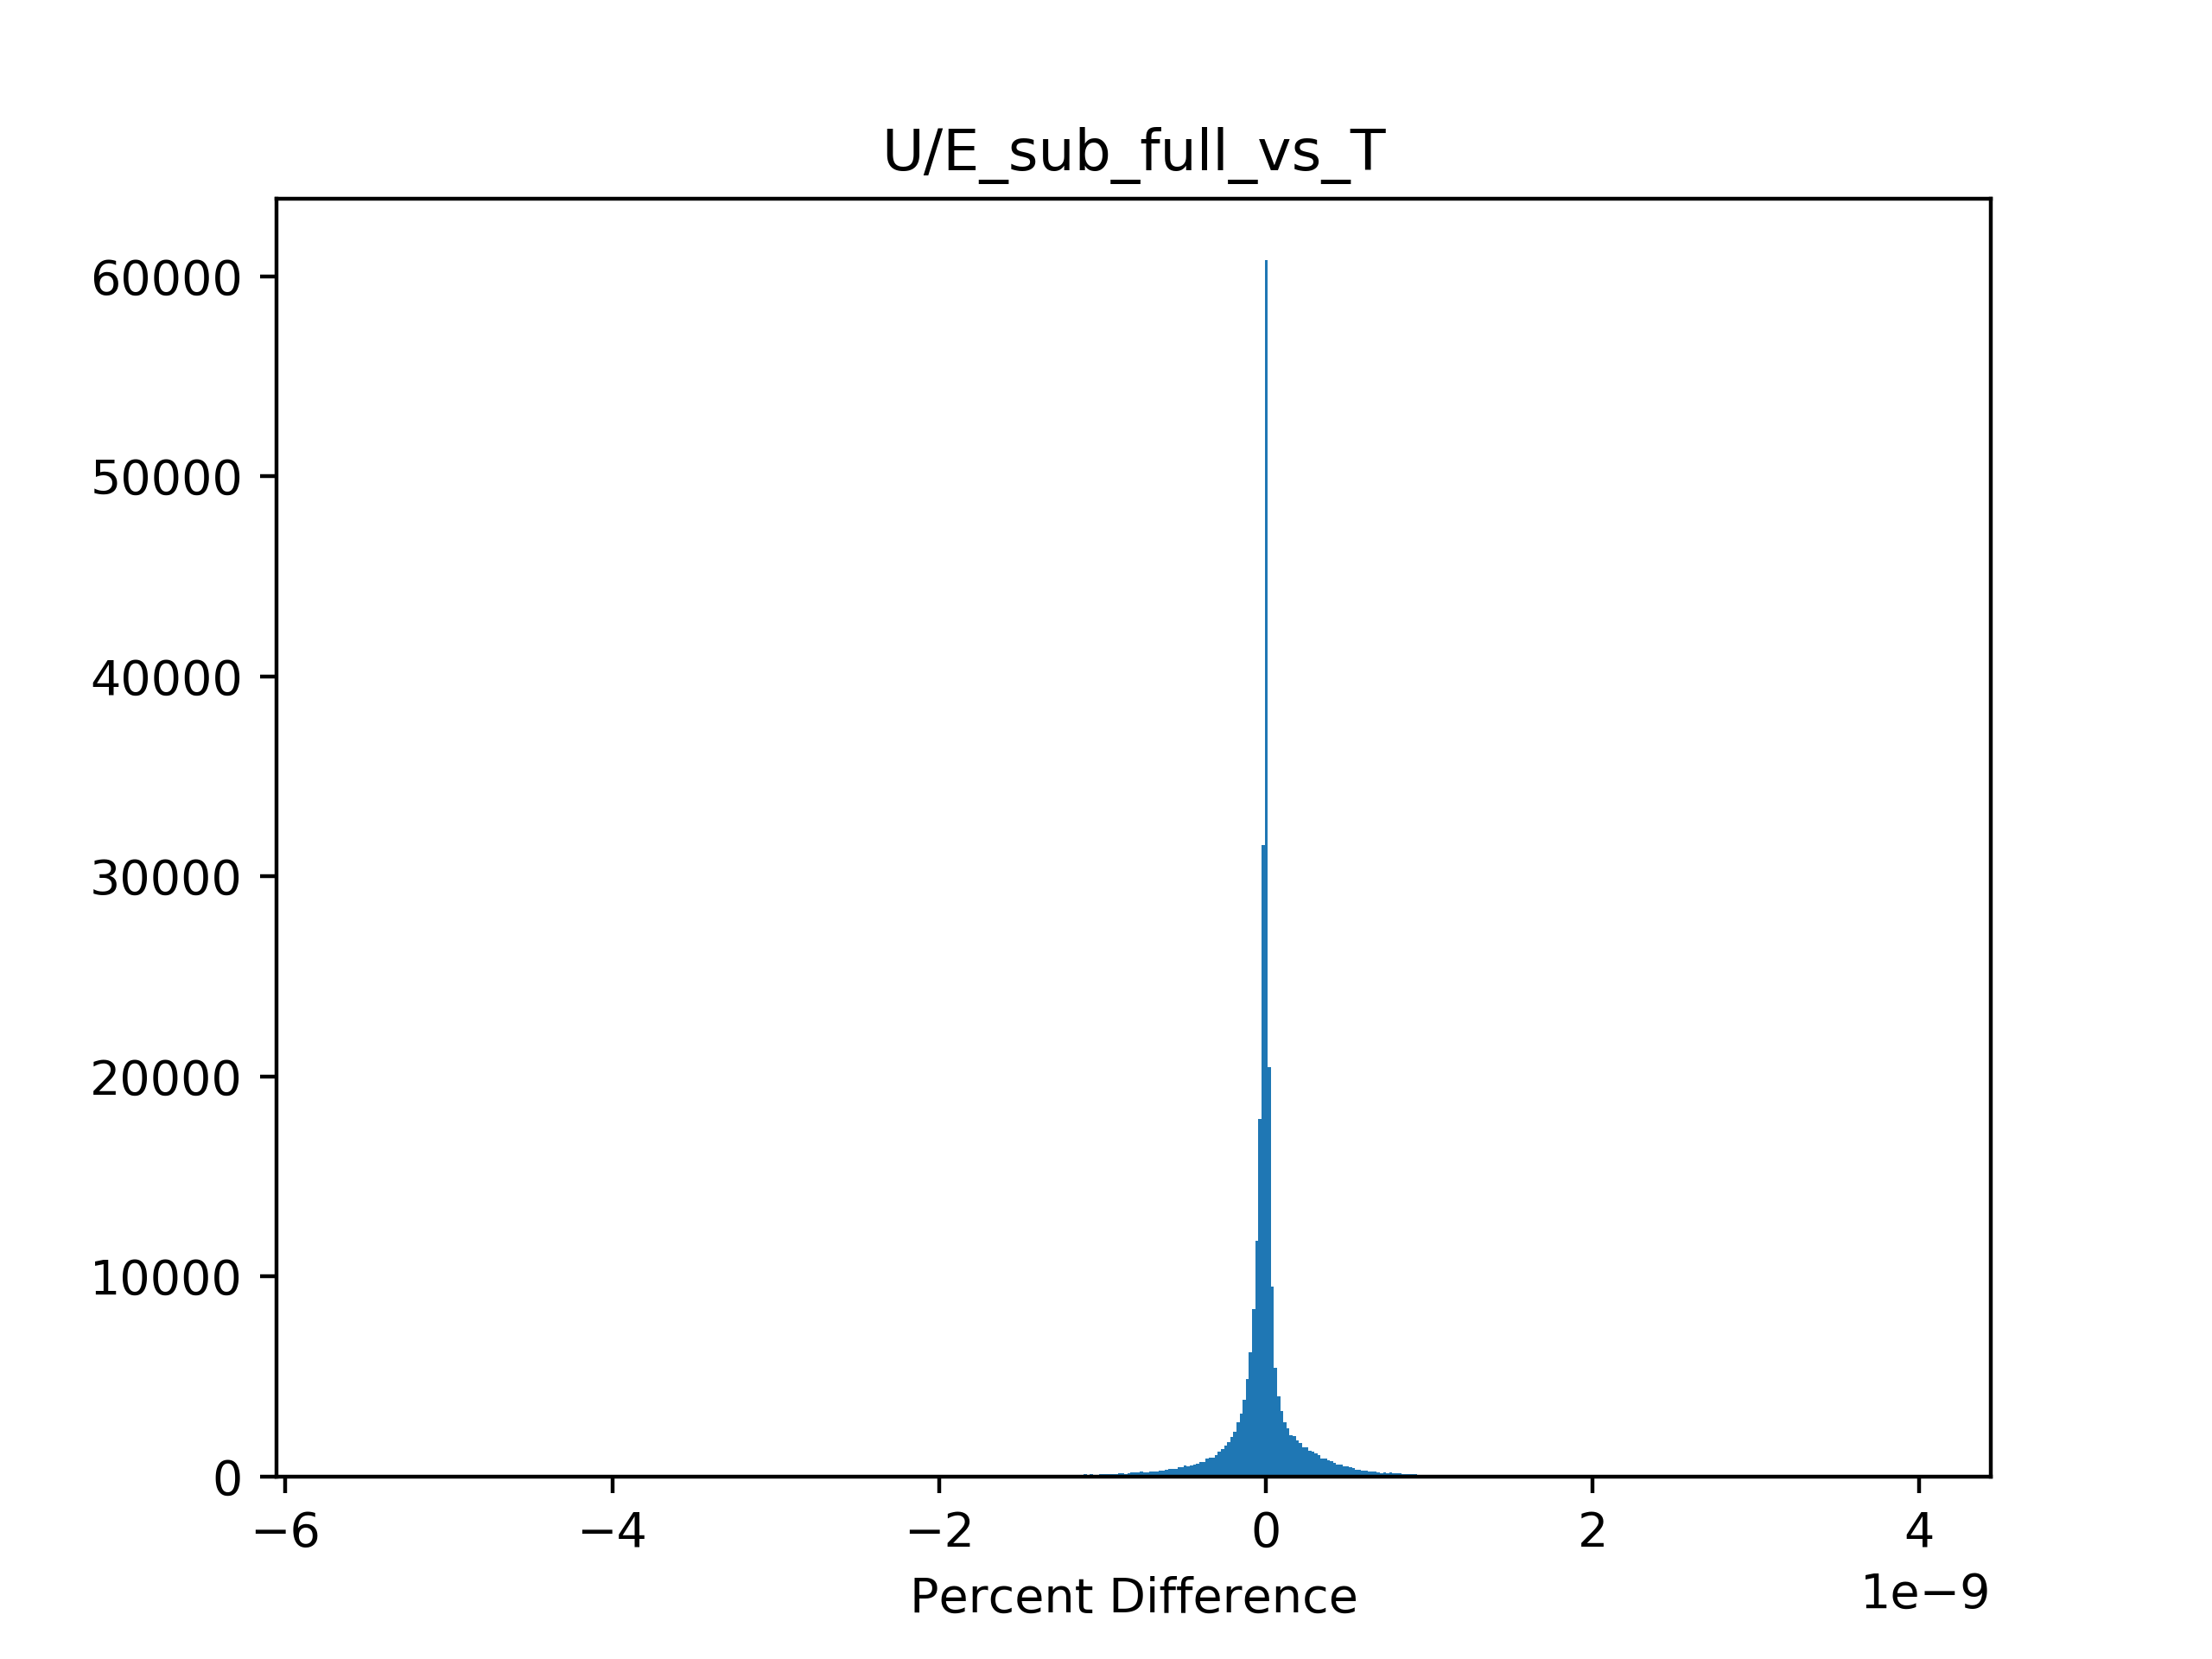
\includegraphics[width=0.8\linewidth]{figs/esub}

    \begin{tabular}{l | c }
    Mean & -1e-11\\
    Absolute value mean: & 1e-10\\
    Max: & 4e-9\\
  \end{tabular}  

    
  \end{frame}
\end{document}

